
\noindent
\begin{tabular}{cc}
\begin{minipage}{0.60\textwidth}
\begin{exerciseS}[Gomito]
Si consideri la corrente stazionaria nel gomito a 90$\,^\circ$ di una 
galleria a vento a circuito chiuso di cui è mostrata in figura la 
sezione nel piano $x$--$y$. Siano assegnate le aree della sezione di 
ingresso, $S_1 = 16 \ m^2$, e di uscita, $S_2 = 56 \ m^2$, 
la portata in volume $Q_1 = 1600 \  m^3/s$ e le pressioni nella 
sezione di ingresso, $P_1 = 1.05 \ bar$, e nella sezione di uscita, 
$P_2 = 1.106 \  bar$. Assumendo che il flusso d'aria sia incomprimibile 
($\rho = 1.225\ kg/m^3$) e che la velocità sulle sezioni di ingresso 
e uscita possa ritenersi uniforme, si determinino le componenti $F_x$ ed 
$F_y$ della spinta che esso esercita sul gomito, usando la convenzione 
indicata in figura.\\
($F_x = 1.876\,10^6\ N$, $F_y = -6.251\,10^6\ N$)
\end{exerciseS}
\end{minipage}
&
\begin{minipage}{0.35\textwidth}
   \begin{center}
   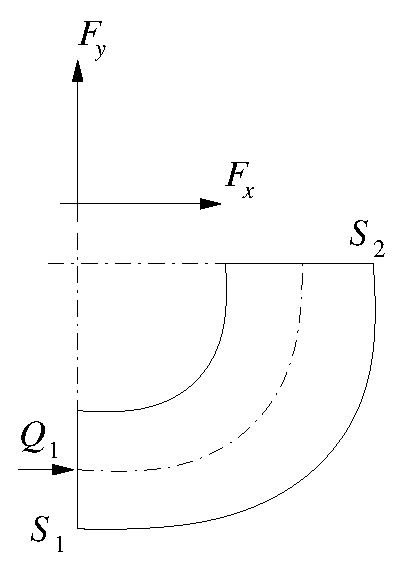
\includegraphics[width=0.60\textwidth]{./fig/gomito_galleria.eps}
   \end{center}
\end{minipage}
\end{tabular}


%%%%%%%%%%%%%%%%%%%%%%%%%%%%%%%%%%%%%%%%%%%%%%%%%%%%%%%%%%%%%%%%%%

\sol

\partone
  Bilanci integrali di massa e quantità di moto.
\begin{equation}
\begin{cases}
  \frac{d}{dt} \int_V \rho = -\oint_{\partial V} \rho \bm{u} \cdot \hat{\bm{n}}  & \text{(massa)} \\
  \frac{d}{dt} \int_V \rho \bm{u} = -\oint_{\partial V} \rho \bm{u} \bm{u} \cdot \hat{\bm{n}}
  +\int_V \bm{f} - \oint_{\partial V} p \hat{\bm{n}} + \oint_{\partial V} {\bm{t}_s} & \text{(quantità di moto)}
\end{cases}
\end{equation}



\parttwo
Vengono fatte alcune ipotesi: regime stazionario, fluido incomprimibile, fluido non viscoso, profili costanti di velocità, no gravità.
Si scrivono i bilanci integrali semplificati, si riconoscono in essi e si calcolano le azioni scambiate con il corpo.

\begin{itemize}
  \item Scrittura dei bilanci integrali con le semplificazioni opportune, derivanti dalle ipotesi.
    \begin{equation}
     \begin{cases}
      \oint_{\partial V} \rho \bm{u} \cdot \hat{\bm{n}} = 0  & \text{(massa)} \\
      \oint_{\partial V} \rho \bm{u} \bm{u} \cdot \hat{\bm{n}} = \oint_{\partial V} \bm{t_n} & \text{(quantità di moto)}
     \end{cases}
    \end{equation}
  \item Ulteriore semplificazione usando l'ipotesi di densità costante e profili di velocità uniformi
    \begin{equation}
     \begin{cases}
      -V_1 A_1 + V_2 A_2 = 0  & \quad \Rightarrow \quad V_1 A_1 = V_2 A_2 = Q \\
      - \rho \vec{V_1} V_1 A_1 + \rho \vec{V_2} V_2 A_2 = \oint_{\partial V} \bm{t_n}
     \end{cases}
    \end{equation}
  \item Relazione tra l'integrale della pressione e la risultante delle forze agenti sul gomito, sfruttando il fatto che l'integrale della normale su tutta la superficie è identicamente nullo. Si identificano con $S_1$ la superficie di ingresso, $S_2$ la superficie di uscita, $S_3$ la superficie laterale.
    \begin{equation}
     \begin{aligned}
      \displaystyle\oint_{S_1\cup S_2\cup S_3} p \hat{n} & =  \displaystyle\oint_{S_1\cup S_2\cup S_3} \bm{t_n} + \displaystyle\oint_{S_1\cup S_2\cup S_3} p_a \hat{n} = \\
      & = -\oint_{S_1} (p-p_a) \hat{n} - \oint_{S_2} (p-p_a) \hat{n} + \underbrace{\oint_{S_3} (\bm{t_n}+p_a\hat{n})}_{=-\bm{f}}  =  \\
      & = -\oint_{S_1} (p-p_a) \hat{n} - \oint_{S_2} (p-p_a) \hat{n} - \bm{f}
     \end{aligned}
    \end{equation}
  \item L'equazione della quantità di moto diventa quindi:
  \begin{equation}
  - \rho \bm{V_1} V_1 A_1 + \rho \bm{V_2} V_2 A_2 = - (p_1 - p_a) A_1 \hat{n}_1 - (p_2 - p_a) A_2 \hat{n}_2 - \bm{F}
  \end{equation}
  \item Proiezione lungo i due assi del sistema di riferimento della risultante delle forze agenti sul gomito.
  Se si considera $p_a = 0$, i risultati numerici sono i seguenti:
  \begin{equation}
  \begin{cases}
    F_x = \rho \frac{Q^2}{A_1} + (p_1 - p_a)A_1  & \quad \Rightarrow \quad   F_x = 1.876 \cdot 10^6 N  \\
    F_y = -  \rho \frac{Q^2}{A_2} - (p_2 - p_a)A_2  & \quad \Rightarrow \quad   F_y =-6.250 \cdot 10^6 N
  \end{cases}
  \end{equation}
\end{itemize}

